%=================================================================
\documentclass[sensors,article,submit,moreauthors,pdftex,10pt,a4paper]{mdpi} 

%=================================================================
%***************** Frizy subfigure *************
\usepackage{subfigure}
%**********************************************
\firstpage{1} 
\makeatletter 
\setcounter{page}{\@firstpage} 
\makeatother 
\articlenumber{x}
\doinum{10.3390/------}
\pubvolume{xx}
\pubyear{2017}
\copyrightyear{2017}
\externaleditor{Academic Editor: name}
\history{Received: date; Accepted: date; Published: date}

%------------------------------------------------------------------
% The following line should be uncommented if the LaTeX file is uploaded to arXiv.org
%\pdfoutput=1

%=================================================================
% Add packages and commands here. The following packages are loaded in our class file: fontenc, calc, indentfirst, fancyhdr, graphicx, lastpage, ifthen, lineno, float, amsmath, setspace, enumitem, mathpazo, booktabs, titlesec, etoolbox, amsthm, hyphenat, natbib, hyperref, footmisc, geometry, caption, url, mdframed, tabto, soul, multirow, microtype, tikz

%=================================================================
%% Please use the following mathematics environments: Theorem, Lemma, Corollary, Proposition, Characterization, Property, Problem, Example, ExamplesandDefinitions, Hypothesis, Remark, Definition
%% For proofs, please use the proof environment (the amsthm package is loaded by the MDPI class).

%=================================================================
% Full title of the paper (Capitalized)
\Title{Development and Testing of a Scene-Compared Convolution Neural Network for Automatic Detection the Damage of Cameras in Monitoring System}



% Author Orchid ID: enter ID or remove command
\newcommand{\orcidauthorA}{0000-0000-000-000X} % Add \orcidA{} behind the author's name
%\newcommand{\orcidauthorB}{0000-0000-000-000X} % Add \orcidB{} behind the author's name

% Authors, for the paper (add full first names)
\Author{Firstname Lastname $^{1,\dagger,\ddagger}$\orcidA{}, Firstname Lastname $^{1,\ddagger}$ and Firstname Lastname $^{2,}$*}

% Authors, for metadata in PDF
\AuthorNames{Firstname Lastname, Firstname Lastname and Firstname Lastname}

% Affiliations / Addresses (Add [1] after \address if there is only one affiliation.)
\address{%
$^{1}$ \quad Affiliation 1; e-mail@e-mail.com\\
$^{2}$ \quad Affiliation 2; e-mail@e-mail.com}

% Contact information of the corresponding author
\corres{Correspondence: e-mail@e-mail.com; Tel.: +x-xxx-xxx-xxxx}

% Current address and/or shared authorship
\firstnote{Current address: Affiliation 3} 
\secondnote{These authors contributed equally to this work.}
% The commands \thirdnote{} till \eighthnote{} are available for further notes

% Simple summary
%\simplesumm{}

\abstract{ Multiple cameras monitoring systems are used in many fields. When one or more of the cameras suffer damage, there would inevitably cause some missing of the key information. This paper proposes a novel method based deep convolutional neural networks (DCNN) to real-time detect the work situation of the cameras in a whole day. Different from previous DCNN which the net input only one image and output the classified label, show the camera is damaged or not, the proposed method input all of the cameras' images at once, those images are taken by the cameras in the same scene, then concatenate those images in their channel dimensionality, the process of the net can compare these images and readily find the abnormal cameras. The experiments and results demonstrate that the proposed method is not only able to attain a higher accuracy but convergence faster.}

% Keywords
\keyword{convolutional neural networks; multiple cameras; damage detection; scene compare}

% The fields PACS, MSC, and JEL may be left empty or commented out if not applicable
%\PACS{J0101}
%\MSC{}
%\JEL{}

%%%%%%%%%%%%%%%%%%%%%%%%%%%%%%%%%%%%%%%%%%
% Only for journal Applied Sciences:
%\featuredapplication{Authors are encouraged to provide a concise description of the specific application or a potential application of the work. This section is not mandatory.}
%%%%%%%%%%%%%%%%%%%%%%%%%%%%%%%%%%%%%%%%%%


%%%%%%%%%%%%%%%%%%%%%%%%%%%%%%%%%%%%%%%%%%
% Only for the journal Data:
%\dataset{DOI number or link to the deposited data set in cases where the data set is published or set to be published separately. If the data set is submitted and will be published as a supplement to this paper in the journal Data, this field will be filled by the editors of the journal. In this case, please make sure to submit the data set as a supplement when entering your manuscript into our manuscript editorial system.}

%\datasetlicense{license under which the data set is made available (CC0, CC-BY, CC-BY-SA, CC-BY-NC, etc.)}

%%%%%%%%%%%%%%%%%%%%%%%%%%%%%%%%%%%%%%%%%%
% For Conference Proceedings Papers:
%\conferencetitle{Add the conference title here}

%\setcounter{secnumdepth}{4}
%%%%%%%%%%%%%%%%%%%%%%%%%%%%%%%%%%%%%%%%%%

\begin{document}
%%%%%%%%%%%%%%%%%%%%%%%%%%%%%%%%%%%%%%%%%%
%% Only for the journal Gels: Please place the Experimental Section after the Conclusions

%%%%%%%%%%%%%%%%%%%%%%%%%%%%%%%%%%%%%%%%%%

%\section{Introduction}
%
%The introduction should briefly place the study in a broad context and highlight why it is important. It should define the purpose of the work and its significance. The current state of the research field should be reviewed carefully and key publications cited. Please highlight controversial and diverging hypotheses when necessary. Finally, briefly mention the main aim of the work and highlight the principal conclusions. As far as possible, please keep the introduction comprehensible to scientists outside your particular field of research. Citing a journal paper \cite{ref-journal}. And now citing a book reference \cite{ref-book}. Please use the command \citep{ref-journal} for the following MDPI journals, which use author-date citation: Administrative Sciences, Arts, Econometrics, Economies, Genealogy, Humanities, IJFS, JRFM, Laws, Religions, Risks, Social Sciences.
\section{Introduction}

Surveillance cameras can be seen in everythere, schools, communities, markets and highway. All of these automated detetion systems, based on multi cameras, constitute an intelligent society. Some of the cameras are damaged will inevitably cause blind spots, as a result some scene information is missing and the function of the monitoring system is affected. Therefore, if the maintenance personnel be informed at the first time when the some of the cameras are damaged, the camera can be repaired at once and the loss will be minimized.

Currently, surveillance cameras can dignose the shelter, which make the image become blur because the lens is covered and is not in focus state (Figure \ref{shelter}). Through filter the image by laplacian operator, and then computer the average variance of the image matrix. If the result value less than a setted threshold meaning the image is blur and camera is convered by something. However, when lens is partially blocked, local damaged or the camera is subject to signal interference, the image shown as in Figure \ref{blindSpotFigure}, will also cause monitoring blind spots, the algorithm needs to be detected this situation in real time. As the local blind spot's shape, color and location in the pictures are random and varied, it is difficult that use the features constructed by human to identify the damaged images. A well solution is that using deep convolution neural networks to classify these images to different category. DCNN trained by supervision method with substantial labeled images, can automaticlly learn to extract image feature \cite{zeiler2014visualizing}. DCNN has the capability to learning hierarchical representations, it can fuse input data and extract basic features in the lower layers, fuse basic features into high level features and decisions in the middle layers, and further fuse these features and decisions in the higher layers to obtain the final diagnosis result.

\begin{figure}[H]
\centering
\subfigure[]{
	\label{Fig.sub.1}
	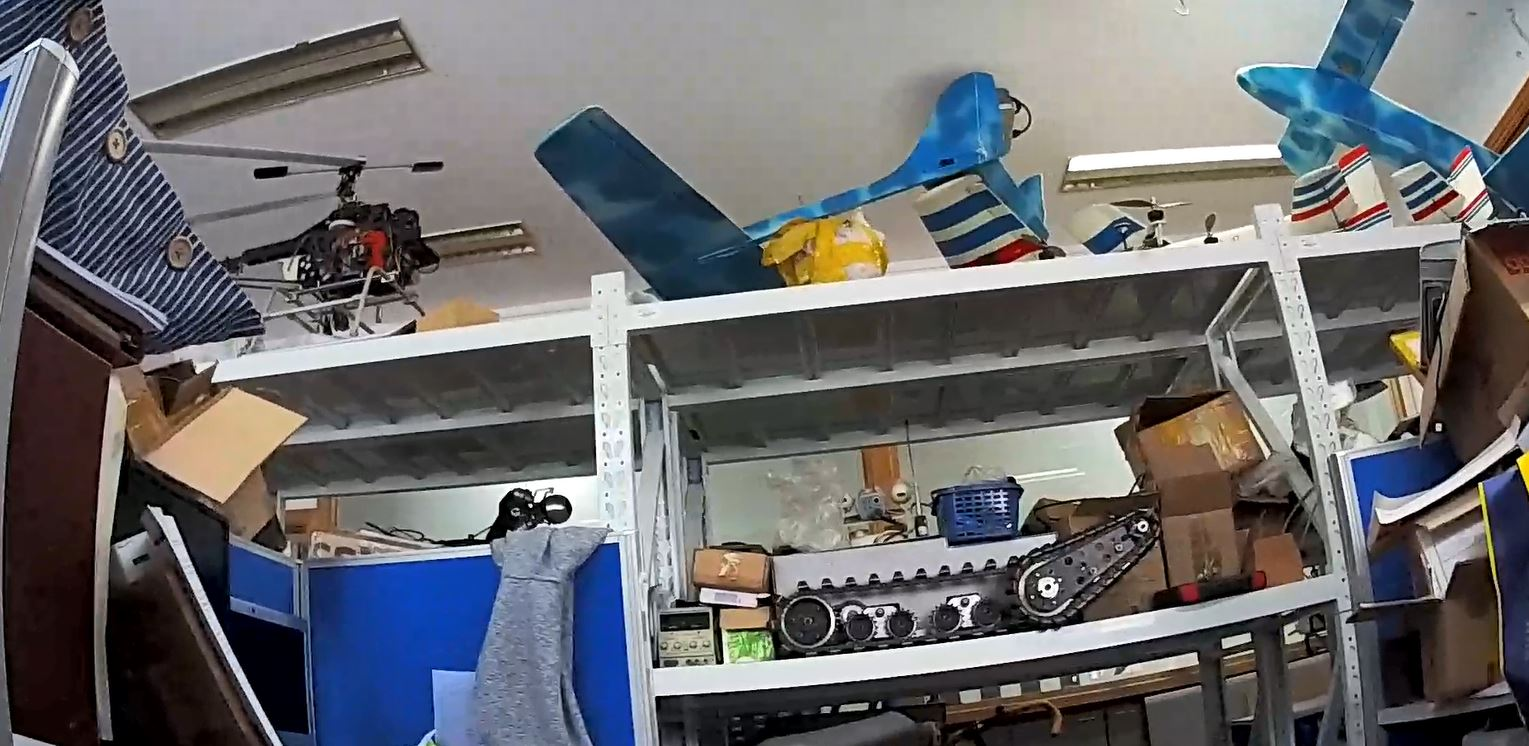
\includegraphics[width=5 cm]{1-1.JPG}
}
\subfigure[]{
	\label{Fig.sub.2}
	
\includegraphics[width=5 cm]{1-2.JPG}
}
\subfigure[]{
	\label{Fig.sub.3}
	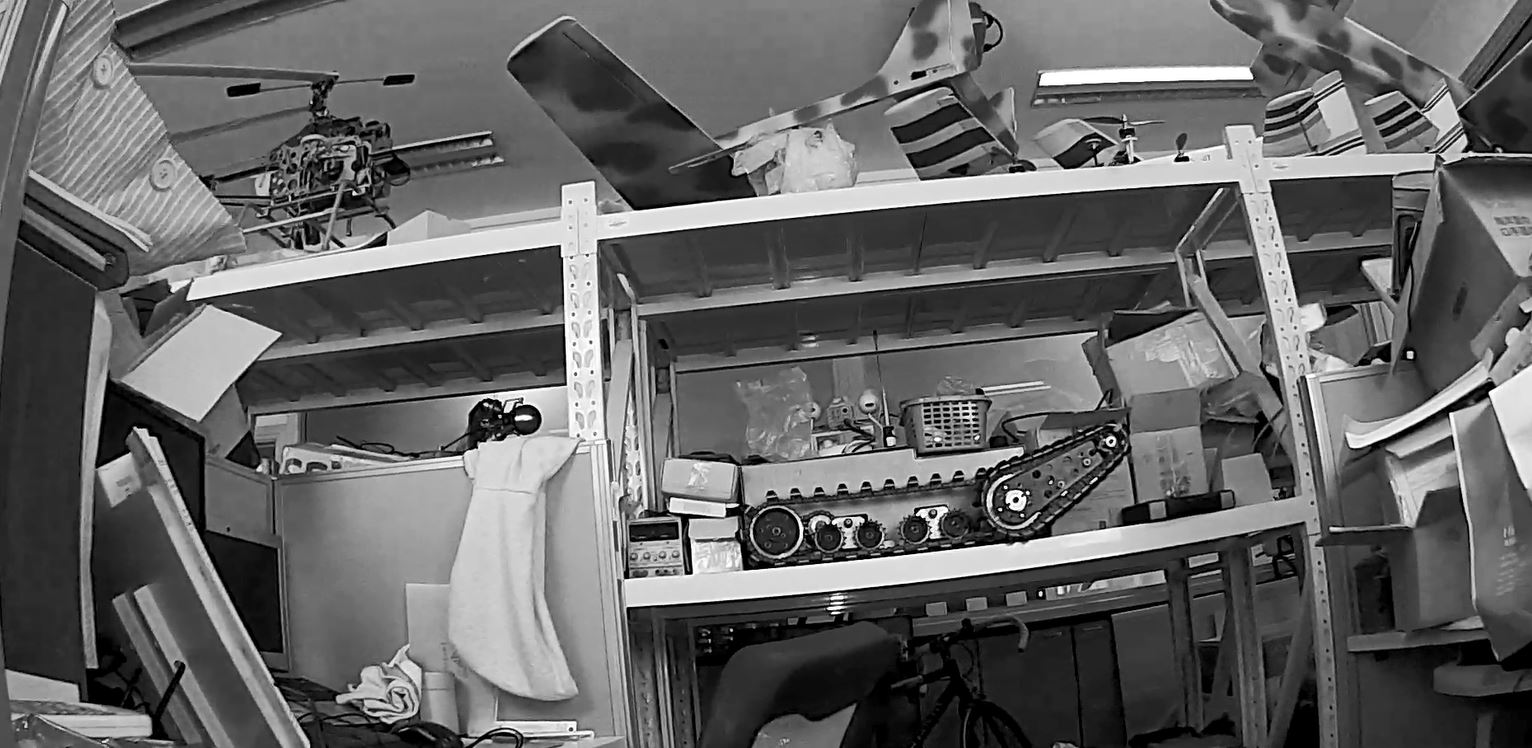
\includegraphics[width=5 cm]{1-3.JPG}
}
\subfigure[]{
	\label{Fig.sub.4}
	
\includegraphics[width=5 cm]{1-4.JPG}
}
\caption{Examples of the normal images and lens covered images. (\textbf{a}) and (\textbf{b}) show a normal surveillance camera image taked in daytime and a image taked when the lens is covered by a piece of cloth. (\textbf{c}) and (\textbf{d}) show a normal surveillance camera image taked in night by Near-Infrared and a image taked when the lens is covered by a piece of cloth.}
\label{shelter}
\end{figure} 

\begin{figure}[H]
\centering
\subfigure[]{
	\label{Fig.sub.1}
	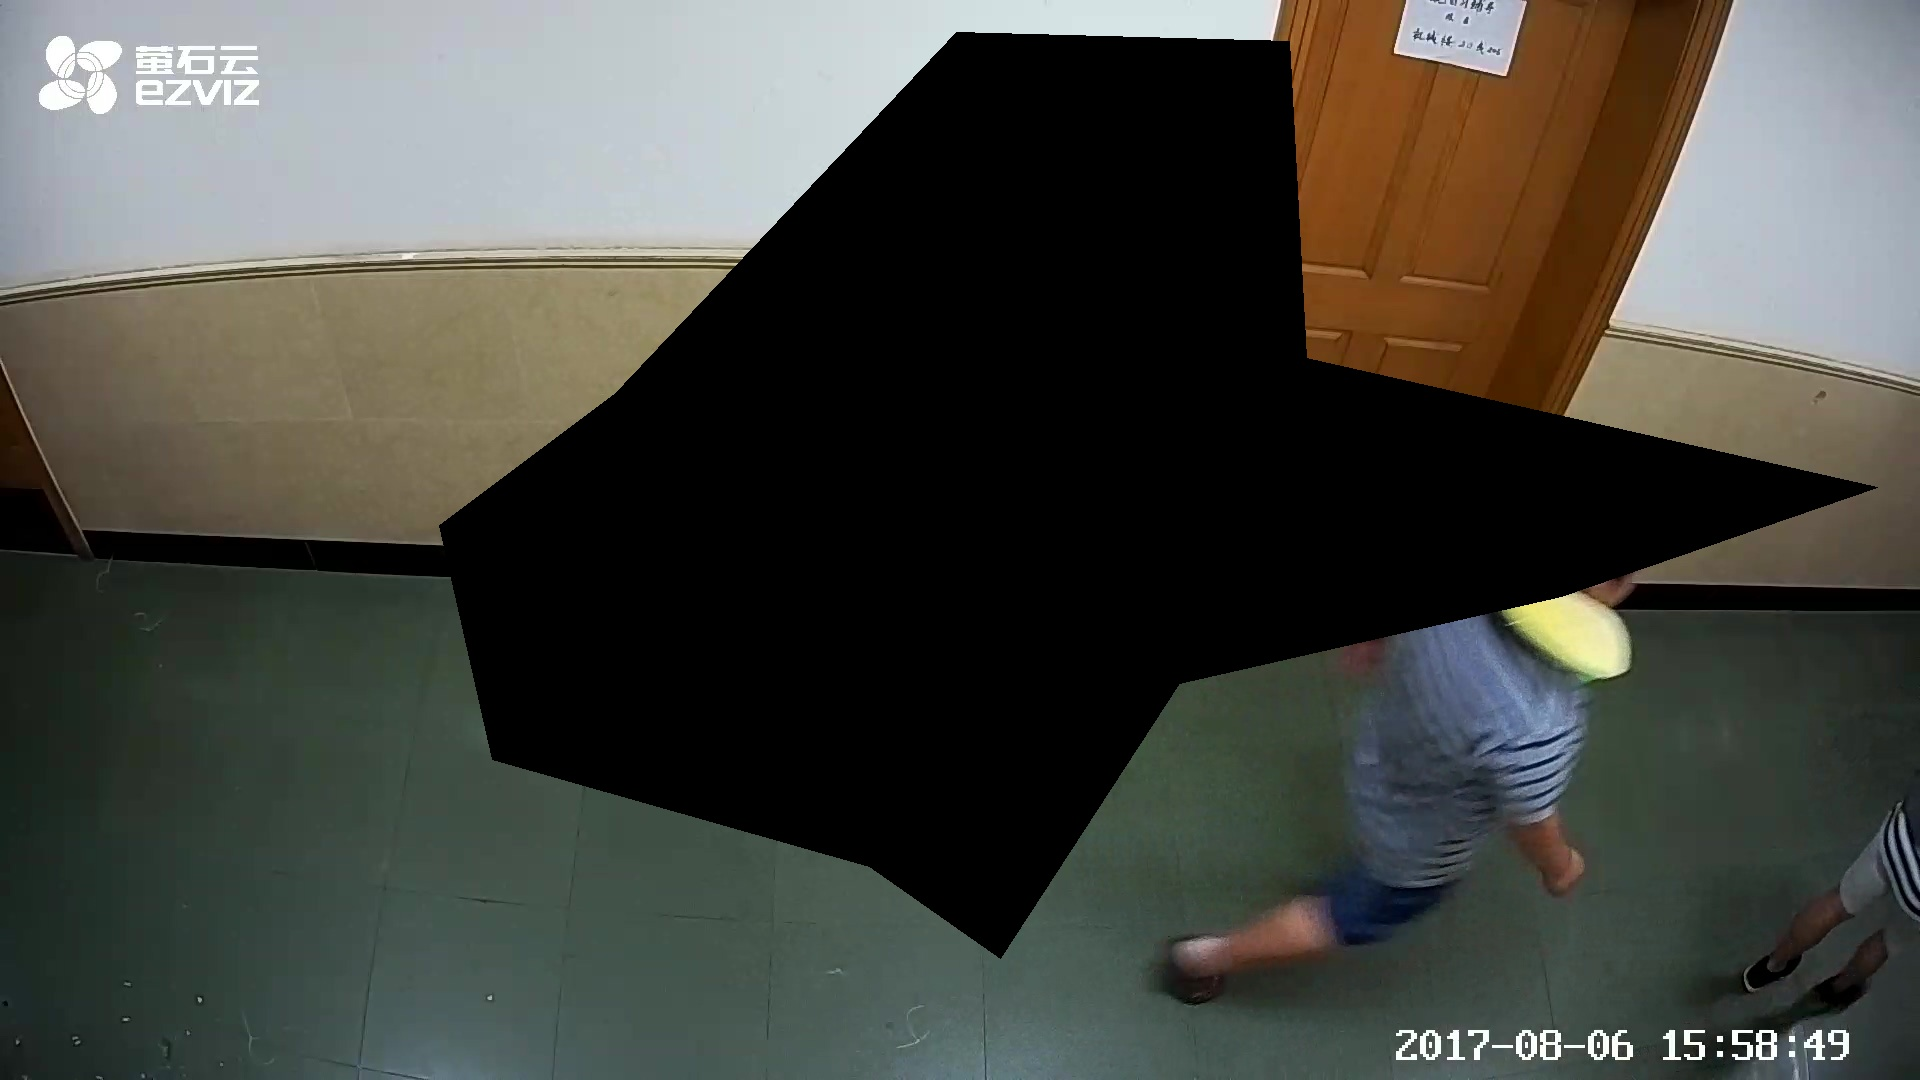
\includegraphics[width=5 cm]{2-1.jpg}
}
\subfigure[]{
	\label{Fig.sub.2}
	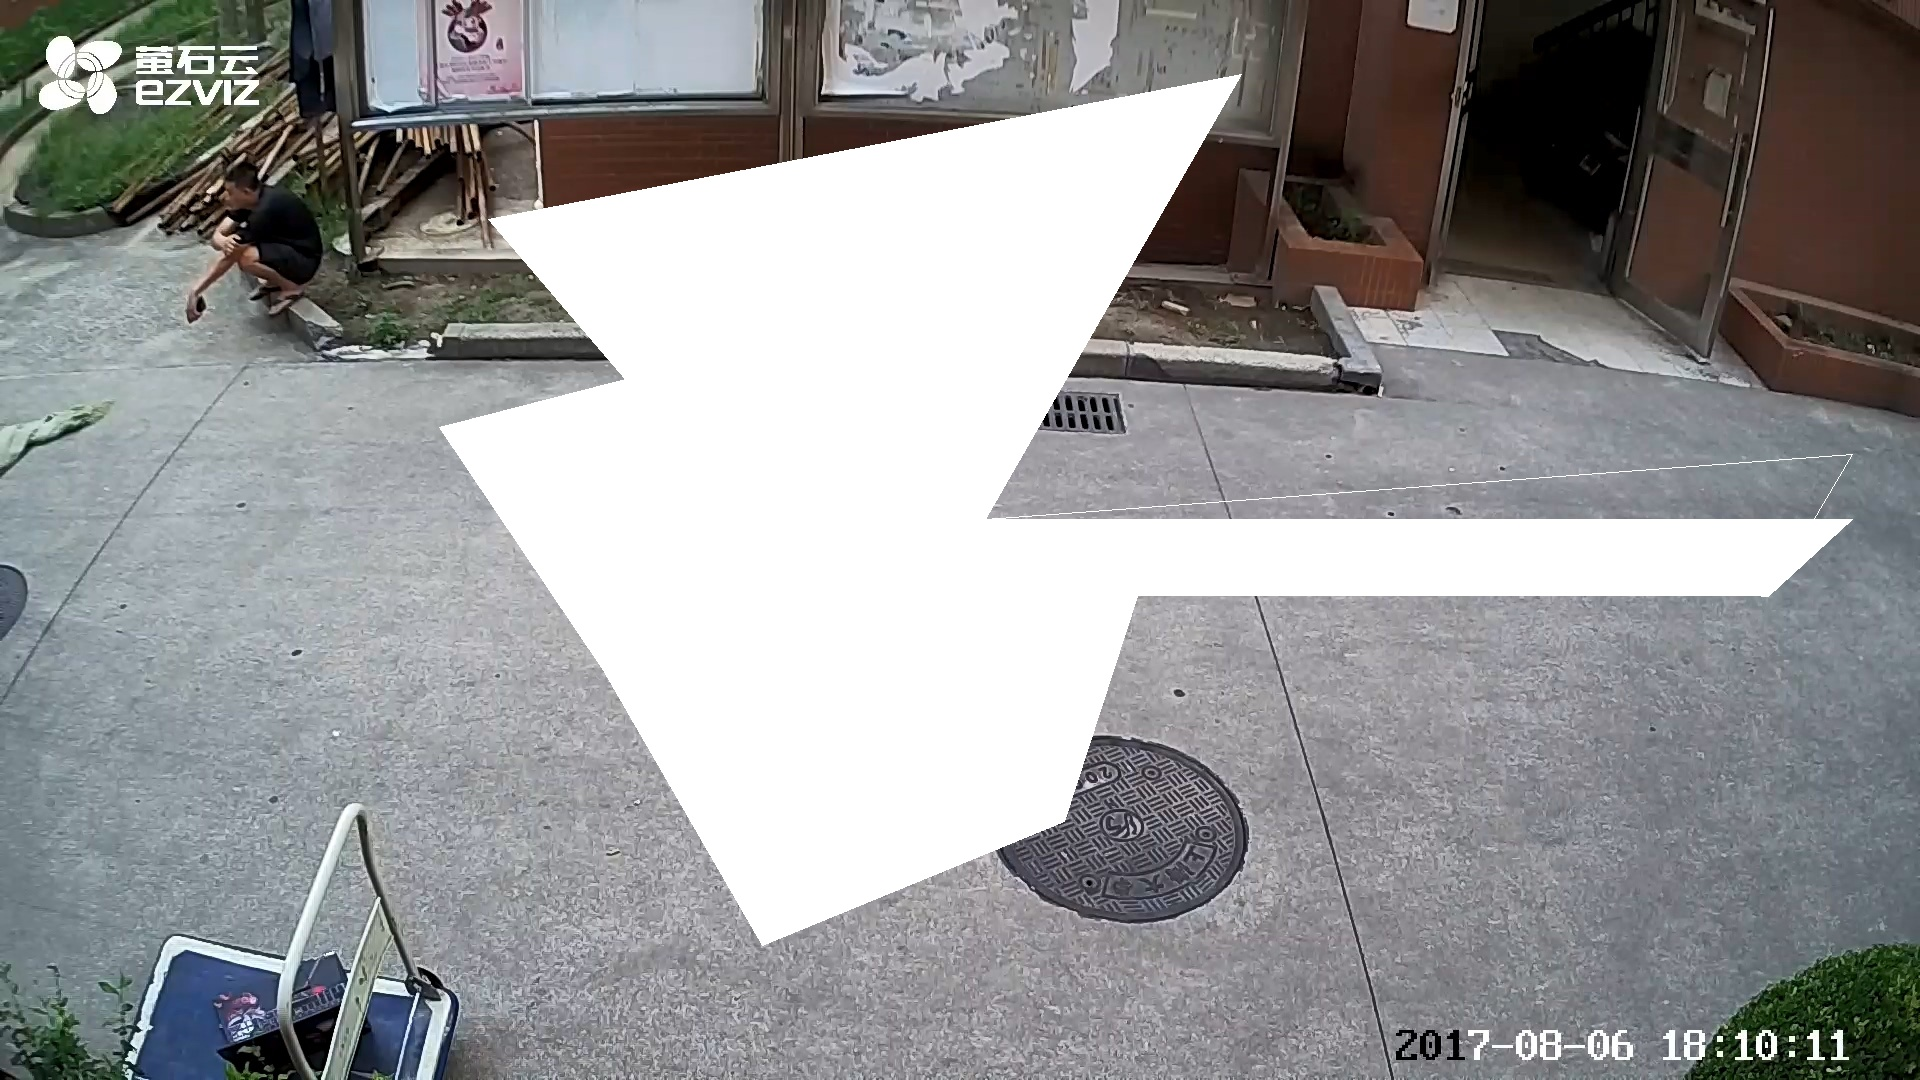
\includegraphics[width=5 cm]{2-2.jpg}
}
\subfigure[]{
	\label{Fig.sub.3}
	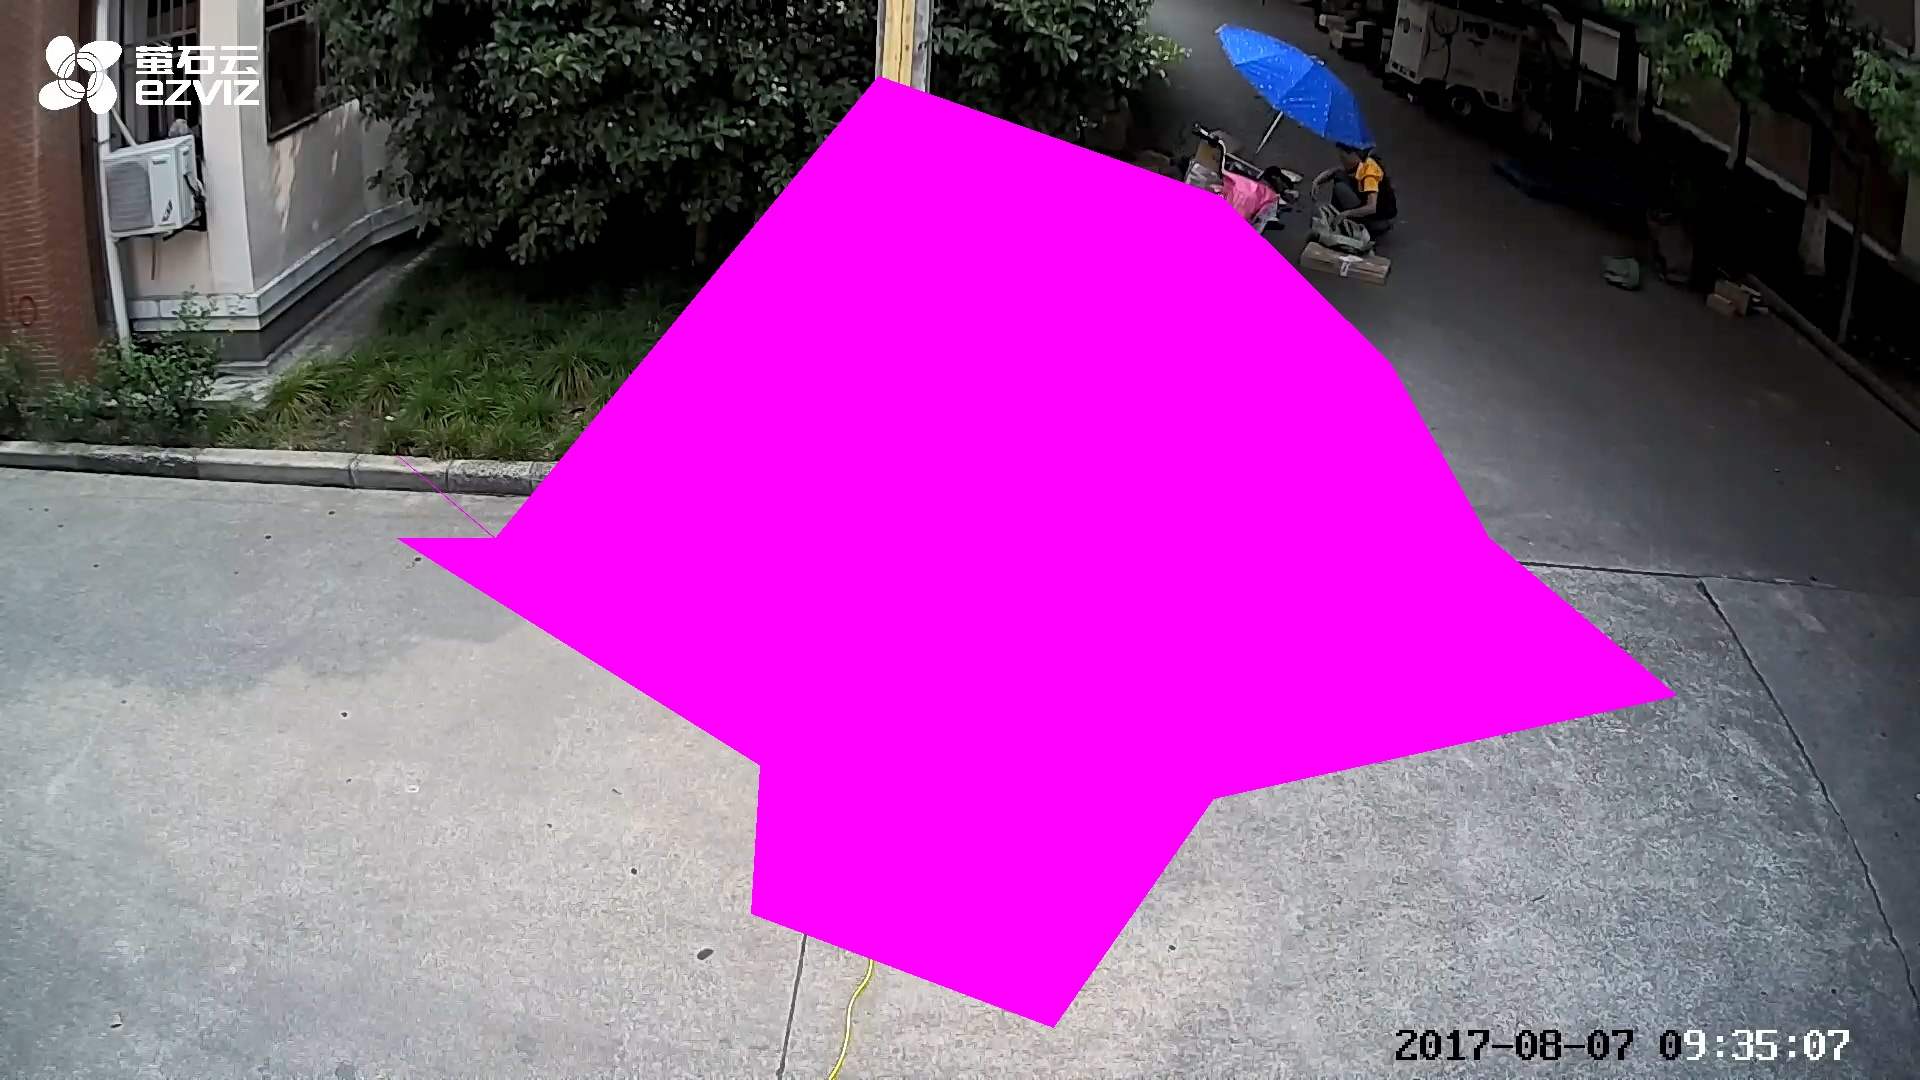
\includegraphics[width=5 cm]{2-3.jpg}
}
\subfigure[]{
	\label{Fig.sub.4}
	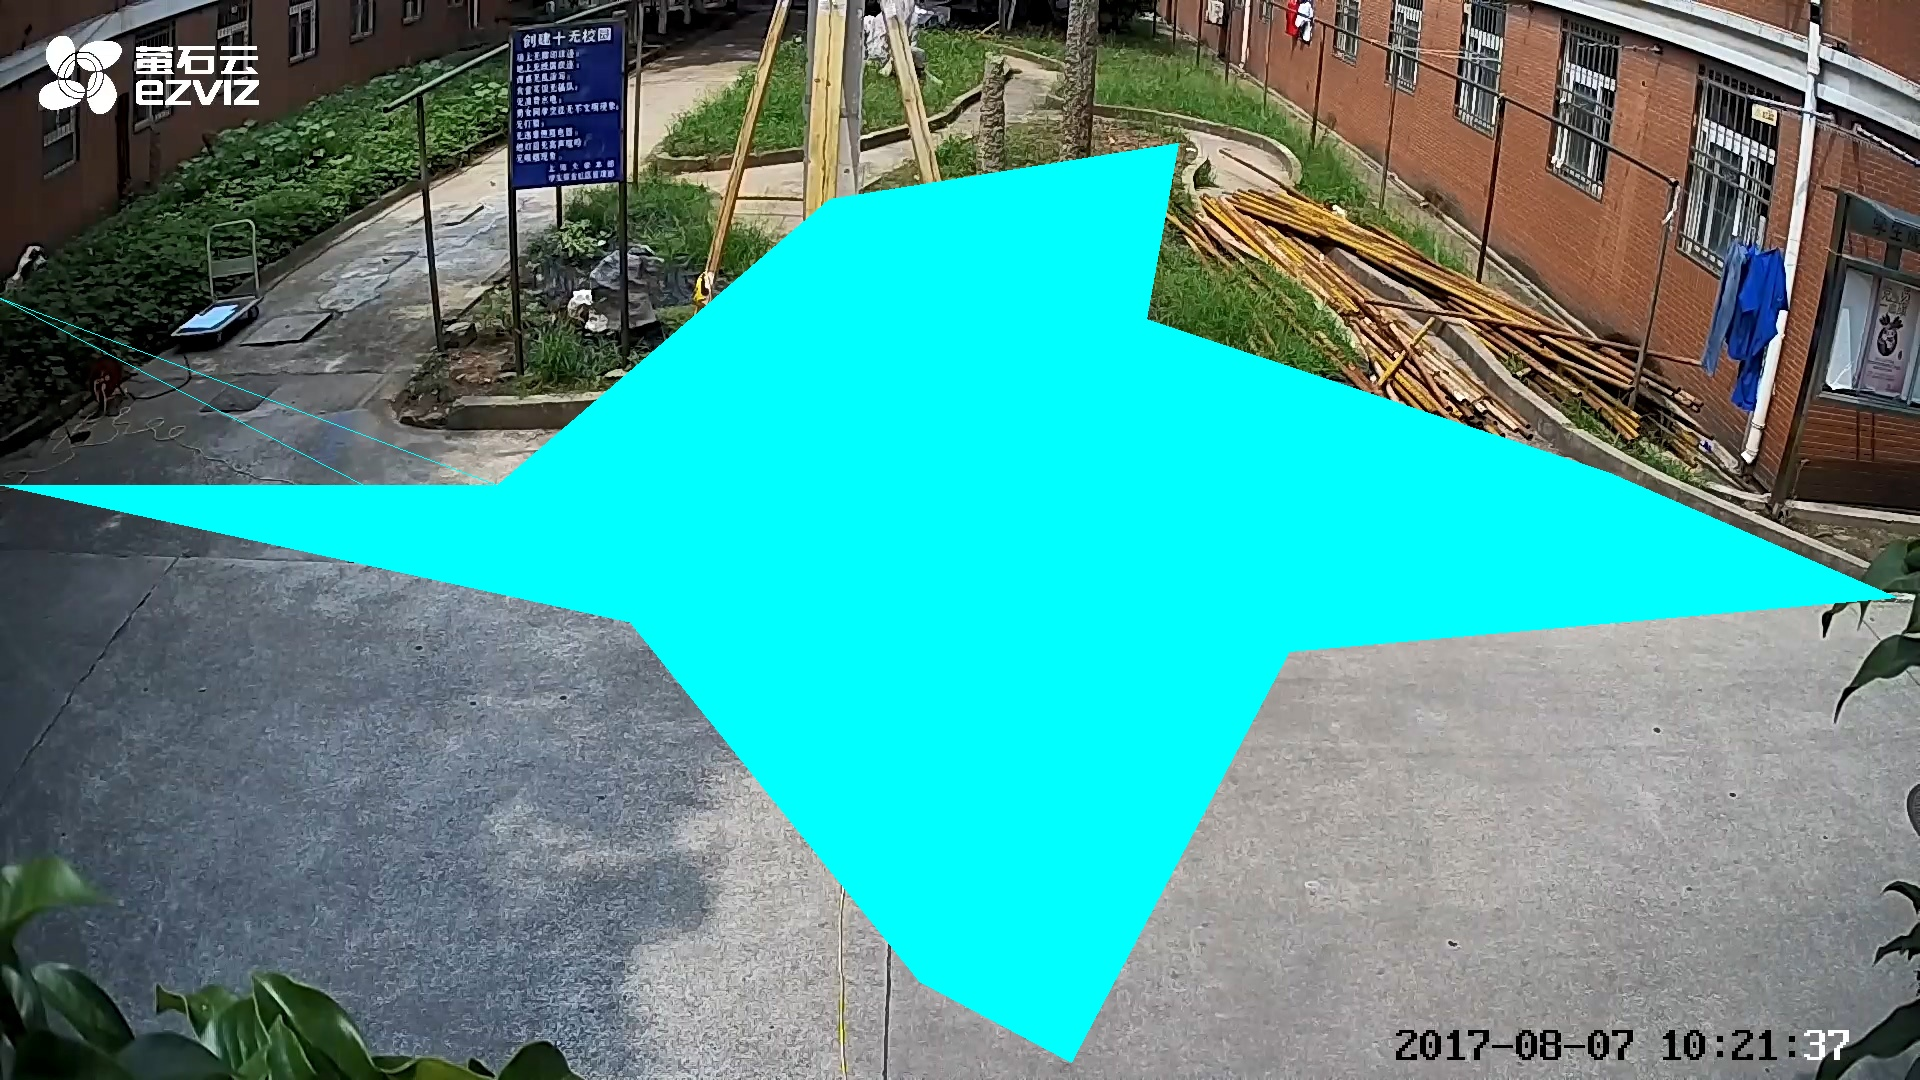
\includegraphics[width=5 cm]{2-4.jpg}
}
\caption{Examples of the blind spot images, which the spot's shape, color and location in images are diverse.}
\label{blindSpotFigure}
\end{figure} 

Since 2012 Alexnet won the Imagenet \cite{imagenet} title with a higher accuracy than the second \cite{AlexNet}, DCNN has been used in many areas, such as bearing fault diagnosis \cite{BearingFaultDiagnosis}, traffic prediction \cite{TrafficPrediction}, fruit detection \cite{FruitDetection} and et al. The common characteristics of above DCNN input is only one image, the network can extract the image feature and match it with the trained feature to identify the image. However, In multiple cameras monitoring system, for example in crossroads traffic monitoring system, cameras are in the same brightness, background and scene, when a camera is damaged, the image feature is significantly different from others. We can use this attribute to help us find out the damaged camera. So, we proposed a kind of convolution network, the main feature is that the network has multiple input, can compare these input cameras' images and real-time distinguish the damaged image. We call it Scene-Compared Convolution Neural Network. The proposed method input all of the cameras' images at once, those images are taken by the cameras in the same scene, then concatenate these images in their channel dimensionality, the process of the network can compare these images and readily find the abnormal cameras. The contributions of this paper are therefore:
\begin{itemize}[leftmargin=*,labelsep=5.8mm]
	\item	We proposed a Scene-Compared Convolution Neural Network that can readily discern the damaged cameras in multiple cameras monitoring system.
	\item	The proposed network converges faster and has higher accuracy than other network architecture.
	\item	We visualized the feature map of the network learned, proved the reason of the high-performance of the Scene-Compared Network architecture.
\end{itemize}

The rest of the paper is organized as follows: In Section 2, a two-step Scene-Compared Network that includes concatenating all cameras images to one in their channel dimensionality and some common CNN layers to process the "big image". In Section 3, experiments are conducted on the proposed Scene-Compared network, and are compared with the other prevailing methods. Finally, conclusions are drawn with future study directions in Section 4. 

%%%%%%%%%%%%%%%%%%%%%%%%%%%%%%%%%%%%%%%%%%
\section{Methods}

In the monitoring system, the camera images data distribution are highly similarity, so we construct the Scene-Compared Network. First, converting all images to one "big image". Then process the this "big image" with the common DCNN methods. Figure \ref{Scene-ComparedNetArchitecture} illustrates the architecture of the proposed network. We will demonstrate the advantages of this architecture in the experiment section. 
\begin{figure}[H]
	\centering
	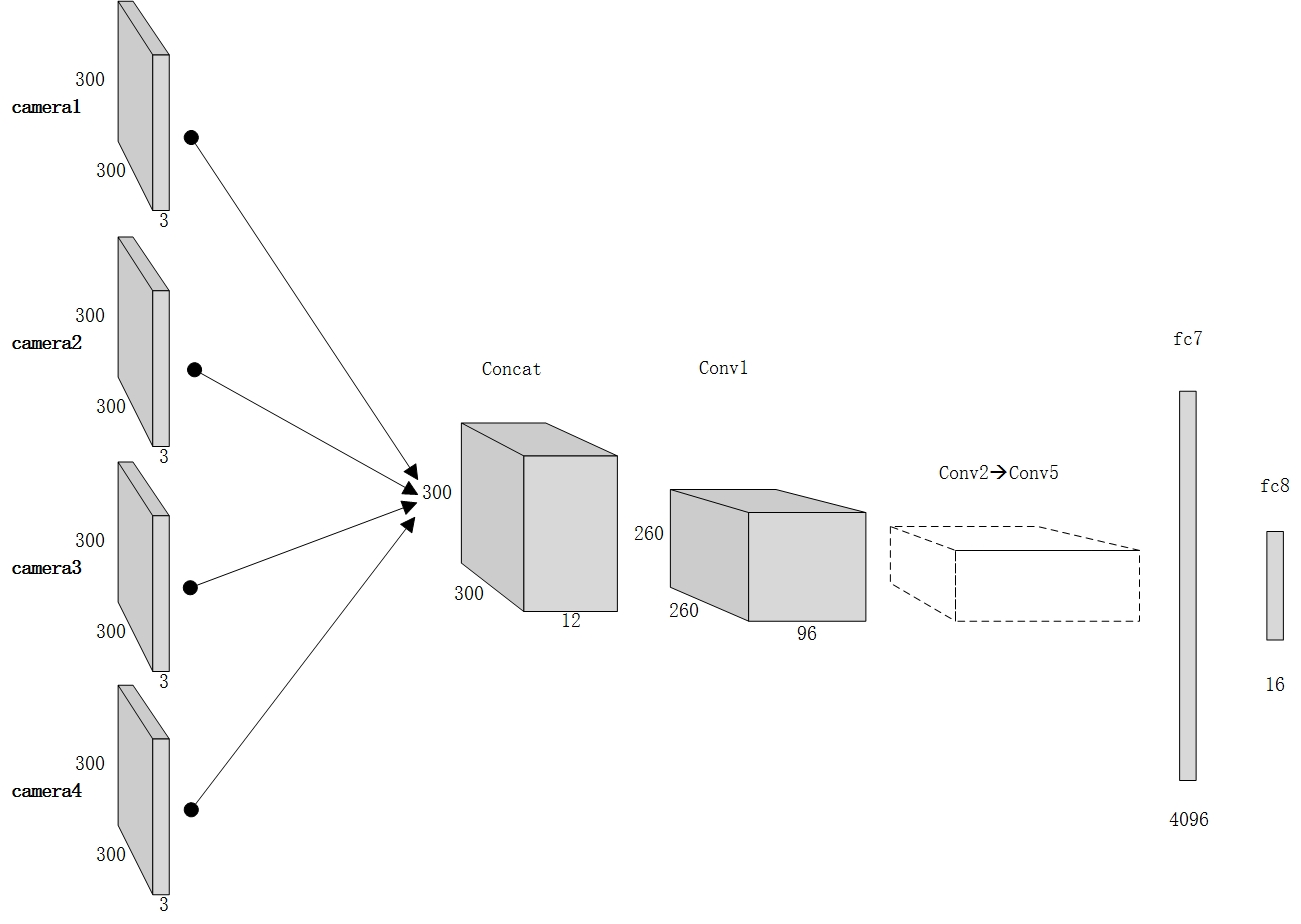
\includegraphics[width=15 cm]{3.jpg}
	\caption{The Scene-Compared Network architecture.}
	\label{Scene-ComparedNetArchitecture}
\end{figure}

%%%%%%%%%%%%%%%%%%%%%%%%%%%%%%%%%%%%%%%%%%
\subsection{Converting all images to one}

As Figure \ref{Scene-ComparedNetArchitecture} illustrated, The network input all of the cameras' images at once, then concatenate these images in their channel dimensionality. Let $M_{ij}^{mn}$ represent the $m$th camera image, $n$th channel, $i$th row, $j$th column pixel, then we denote the "big image" matrix by:

\begin{equation}
\begin{bmatrix}
M_{i,j}^{11},M_{i,j}^{12},M_{i,j}^{13},M_{i,j}^{21},...,M_{i,j}^{m1},M_{i,j}^{m2},M_{i,j}^{m3}
\end{bmatrix}
\end{equation}

In the training phase, label of the "big image" is decided by all labels of the source images, which label1 to lable4 respectively represent the camera1 to camera4. The number zero means the camera is operating well and number one means the camera is damaged, the image has some defect areas. The merge rules are showed in Table \ref{LabelsMergeRules}.According to the original images' label which compose the "big image", the label of the "big image" id divided into sixteen categories.

\begin{table}[H]
\caption{Labels merge rules.}
\centering
%% \tablesize{} %% You can specify the fontsize here, e.g.  \tablesize{\footnotesize}. If commented out \small will be used.
\begin{tabular}{cccc|c}
\toprule
\textbf{label 1}	& \textbf{label 2}	& \textbf{label 3}	& \textbf{label 4}	& \textbf{result label}\\
\midrule
0		& 0			& 0				&0					&0\\
1		& 0			& 0				&0					&1\\
0		& 1			& 0				&0					&2\\
0		& 0			& 1				&0					&3\\
0		& 0			& 0				&1					&4\\
1		& 1			& 0				&0					&5\\
1		& 0			& 1				&0					&6\\
1		& 0			& 0				&1					&7\\
0		& 1			& 1				&0					&8\\
0		& 1			& 0				&1					&9\\
0		& 0			& 1				&1					&10\\
1		& 1			& 1				&0					&11\\
1		& 1			& 0				&1					&12\\
1		& 0			& 1				&1					&13\\
0		& 1			& 1				&1					&14\\
1		& 1			& 1				&1					&15\\
\bottomrule
\end{tabular}
\label{LabelsMergeRules}
\end{table}

\begin{equation}
Big\ image\ label = rules\{labe1_1, label_2, ..., label_m\}
\end{equation}

\subsection{CNN Process}
 
CNN Process include convolutional layer, active layer, pooling layer, and fully connected layer. It caculates the classification loss, throught back propagation and gradient descent to adjust the weights of the convolution kernels to make the kernels learn to extraction useful features. In the following part, we will describe these kinds of layers in more detail. 

Convolutional layer is composed of a number of two-dimensional filters, each of the filters is a feature extractor. Suppose the input of the convolutional layer is $X^{N_{in} \times W_{in} \times H_{in}}$, meaning there are $N_{in}$ channels, each of the channels' width is $W_{in}$, height is $H_{in}$. If the convolutional layer has $n$ filters, the dimensional of thess filters are $w \times h$, then the output of the convolutional layer can be calculated as follows\cite{ConvolutinFormula}:

\begin{equation}
C_j = \sum_{i=1}^{N_{in}}X_i*W_j + B_j
\end{equation}
where $C_j$ is the $j$-th channel of the convolutional layer; $X_i$ represents the input data of the $i$-th channel; $W_j$ is the weight of $j$-th filter; $*$ is an operator of convolution; $B_j$ denotes the bias of the $j$-th channel. The number of the convolutional layer output channels are equal to the number of the filters. Suppose the convolution padding is $p$, striding is $s$, then the dimensional of the output of the convolutional layer ($N_{out} \times W_{out} \times H_{out}$) can be calculated as follows:

\begin{equation}
N_{out} = n
\end{equation}
\begin{equation}
W_{out} = (W_{in} + 2*p -w) / s + 1
\end{equation}
\begin{equation}
H_{out} = (H_{in} + 2*p -h) / s + 1
\end{equation}

Activation layer as a nonlinear feature, can make the neural network approximate complex function, solve complex problems. It can be represent by the follows:

\begin{equation}
A_{out} = f(A_{in})
\end{equation}
For example, ReLu function\cite{ReLu}: $A(X) = max(0,X)$ .

Pooling layer is a sub-sampling layer, the purpse of this layer is to improves the robustness of learned features through reducing the dimension of the input data. The common used pooling method is max pooling, it outputs only the maximum of each sub-sampling patch of the input channels to reduce the dimension of feature map. The output can be described as follows\cite{ConvolutinFormula}:
\begin{equation}
P_{out} = \max_{Block\in{P_{in}}}\{Block\}
\end{equation}
Suppose the $Block$ size is $s \times s$, this function will pick one max value in each distinct $s$ pooling block in the input data so that the output will become $s$ times smaller along both spatial dimensions.

Fully connected layer is similar a classifier. If previous layers map original data to feature space, fully connected layer plays the role that maps the feature space to sample labeled space. Typically, using the softmax regression to learn the classifier distribution. Assuming that the task is a $K$-label problem, the output of the softmax
regression can be calculated as follows:

\begin{equation}
P_j = \frac{e^{z_j}}{\sum_{i=1}^{K}e^{z_i}}
\end{equation}
where $z_j$ denotes the logits of the $j$-th output neuron and $P_j$ denotes the probability of $j$ category.


%%%%%%%%%%%%%%%%%%%%%%%%%%%%%%%%%%%%%%%%%%
\section{Experiments and Results}

\begin{figure}[H]
	\centering
	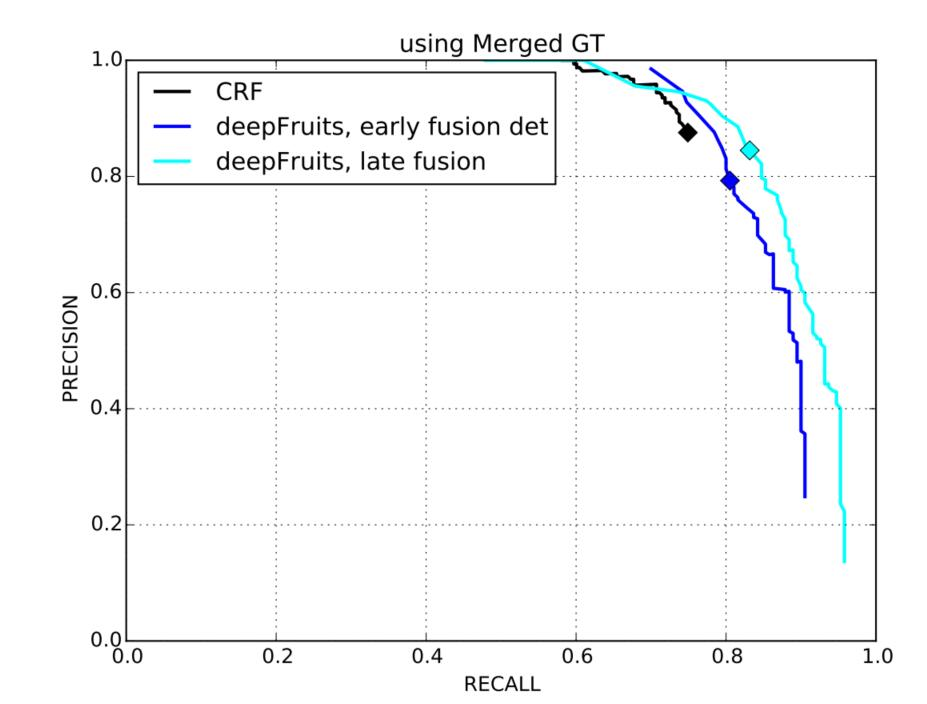
\includegraphics[width=12 cm]{4.jpg}
	\caption{Accuracy of different methods.}
	\label{Scene-ComparedNet}
\end{figure}

\begin{figure}[H]
	\centering
	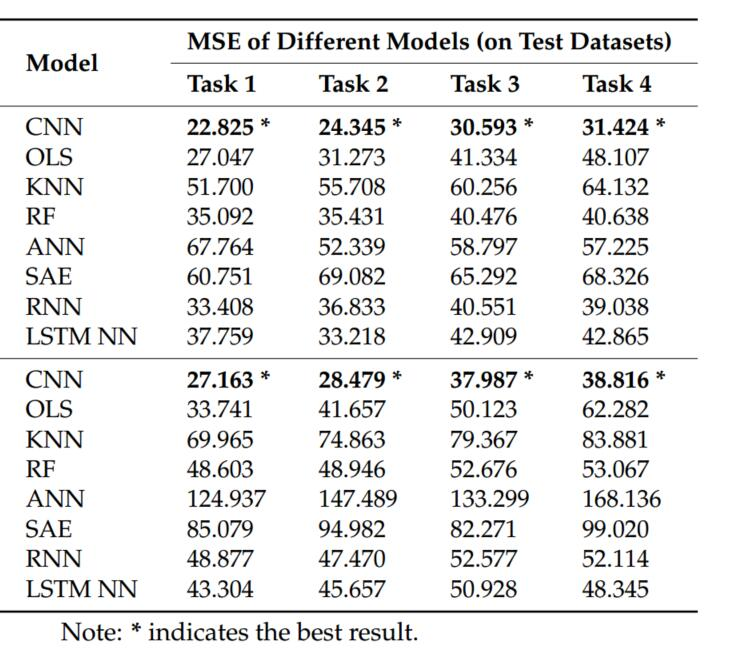
\includegraphics[width=10 cm]{5.jpg}
	\caption{Accuracy on different size of the damage region in the images.}
	\label{Scene-ComparedNet}
\end{figure}

\begin{figure}[H]
	\centering
	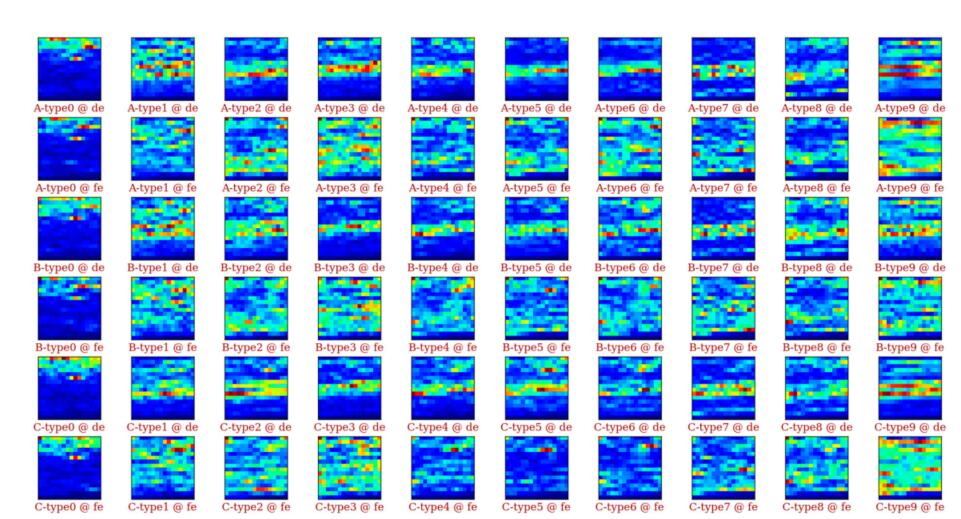
\includegraphics[width=12 cm]{6.jpg}
	\caption{Visualize the feature map of the network.}
	\label{Scene-ComparedNet}
\end{figure}
.

%%%%%%%%%%%%%%%%%%%%%%%%%%%%%%%%%%%%%%%%%%
\section{Conclusions}

The experiments and results demonstrate that the proposed method is not only able to attain a higher accuracy but convergence faster.

%=====================================
% References, variant A: internal bibliography
%=====================================
\begin{thebibliography}{999}
% Reference 1
\bibitem[Zeiler, M.D.; Fergus, R. (2014)]{zeiler2014visualizing}
Zeiler, M.D.; Fergus, R. Visualizing and understanding convolutional networks. {\em ECCV} {\bf 2014}, {\em 2313}, 818--833, DOI.
% Reference 2
\bibitem[A. Berg, J. Deng, and L. Fei-Fei (2010)]{imagenet}
A. Berg, J. Deng, and L. Fei-Fei. Large scale visual recognition challenge 2010. www.image-net.org/challenges. 2010.
% Reference 3
\bibitem[Krizhevsky, Alex, Ilya Sutskever, and Geoffrey E. Hinton (2012)]{AlexNet}
Krizhevsky, Alex, Ilya Sutskever, and Geoffrey E. Hinton. Imagenet classification with deep convolutional neural networks. {\em NIPS} {\bf 2012}.
% Reference 4
\bibitem[Li, Shaobo, et al. (2017)]{BearingFaultDiagnosis}
Li, Shaobo, et al. An Ensemble Deep Convolutional Neural Network Model with Improved DS Evidence Fusion for Bearing Fault Diagnosis. {\em Sensors} {\bf 2017}, {\em 1729}.
% Reference 5
\bibitem[Yu, Haiyang, et al. (2017)]{TrafficPrediction}
Yu, Haiyang, et al. Spatiotemporal Recurrent Convolutional Networks for Traffic Prediction in Transportation Networks. {\em arXiv preprint} {\bf 2017}, {\em 1705.02699}.
% Reference 6
\bibitem[Sa, Inkyu, et al. (2016)]{FruitDetection}
Sa, Inkyu, et al. Deepfruits: A fruit detection system using deep neural networks. {\em Sensors} {\bf 2016}, {\em 1222}.
% Reference 7
\bibitem[Nebauer, C. (1998)]{ConvolutinFormula}
Nebauer, C. Evaluation of convolutional neural networks for visual recognition. {\em IEEE Trans. Neural Netw.} {\bf 1998}, {\em 9}, 685–696.
\bibitem[*******, C. (2011)]{ReLu}
*******, C. Deep Sparse Rectifier Neural Networks. {\em *******. Neural Netw.} {\bf 1998}, {\em 9}, 685–696.
\end{thebibliography}

% The following MDPI journals use author-date citation: Arts, Econometrics, Economies, Genealogy, Humanities, IJFS, JRFM, Laws, Religions, Risks, Social Sciences. For those journals, please follow the formatting guidelines on http://www.mdpi.com/authors/references
% To cite two works by the same author: \citeauthor{ref-journal-1a} (\citeyear{ref-journal-1a}, \citeyear{ref-journal-1b}). This produces: Whittaker (1967, 1975)
% To cite two works by the same author with specific pages: \citeauthor{ref-journal-3a} (\citeyear{ref-journal-3a}, p. 328; \citeyear{ref-journal-3b}, p.475). This produces: Wong (1999, p. 328; 2000, p. 475)

%=====================================
% References, variant B: external bibliography
%=====================================
%\externalbibliography{yes}
%\bibliography{your_external_BibTeX_file}

%%%%%%%%%%%%%%%%%%%%%%%%%%%%%%%%%%%%%%%%%%
%% optional
\sampleavailability{Samples of the compounds ...... are available from the authors.}

%%%%%%%%%%%%%%%%%%%%%%%%%%%%%%%%%%%%%%%%%%
\end{document}

